\chapter{Quá trình thực hiện}
\label{Chapter4}

\section{Giới thiệu khái quát}
\par Đề tài \textit{Xây dựng hệ thống theo dõi bệnh nhân từ xa cho người bệnh tăng huyết áp và đái tháo đường} được nhóm thực hiện với mục tiêu xây dựng một hệ thống hỗ trợ bệnh nhân ghi nhận các chỉ số sức khỏe hằng ngày, đồng thời giúp bác sĩ và nhân viên y tế theo dõi tình trạng bệnh nhân thông qua nền tảng web. Ngay từ giai đoạn đầu, nhóm xác định đây là một đề tài có phạm vi tương đối rộng vì hệ thống không chỉ bao gồm một ứng dụng duy nhất, mà cần phát triển đồng thời nhiều thành phần khác nhau như ứng dụng di động cho bệnh nhân và y tá, ứng dụng web cho bác sĩ, trang quản trị cho quản trị viên, hệ thống backend, cơ sở dữ liệu, cơ chế thông báo, xử lý cảnh báo và hạ tầng triển khai trên cloud. Do đó, việc tổ chức quy trình làm việc, phân chia trách nhiệm và lựa chọn công cụ hỗ trợ đóng vai trò rất quan trọng trong toàn bộ quá trình thực hiện.

\par Trong các buổi họp đầu tiên, nhóm đã tiến hành trao đổi về mục tiêu của đề tài, phạm vi chức năng cần hoàn thành, các vai trò người dùng chính trong hệ thống, cách thức lưu trữ dữ liệu sức khỏe và định hướng triển khai thực nghiệm. Nhóm thống nhất rằng hệ thống cần tập trung vào các nghiệp vụ cốt lõi của mô hình Remote Patient Monitoring, bao gồm nhập chỉ số sức khỏe, lưu trữ lịch sử đo, hiển thị xu hướng thay đổi, cấu hình ngưỡng an toàn, sinh cảnh báo khi dữ liệu vượt ngưỡng, gửi nhắc nhở và hỗ trợ trao đổi giữa bệnh nhân với bác sĩ. Bên cạnh đó, nhóm cũng xác định rõ giới hạn của đề tài trong giai đoạn hiện tại là dữ liệu được nhập thủ công, chưa tích hợp trực tiếp với thiết bị IoT và chưa sử dụng các mô hình học máy để dự đoán rủi ro sức khỏe.

\par Sau khi thống nhất định hướng phát triển, nhóm tiến hành lựa chọn các công cụ phục vụ cho quá trình quản lý mã nguồn, quản lý công việc, lưu trữ tài liệu, họp trực tuyến, thiết kế giao diện và vẽ sơ đồ hệ thống. Việc lựa chọn công cụ được cân nhắc dựa trên mức độ quen thuộc của các thành viên, khả năng hỗ trợ làm việc nhóm, tính phù hợp với quy mô đồ án và khả năng ứng dụng trong môi trường phát triển phần mềm thực tế. Các công cụ được nhóm sử dụng bao gồm GitHub Organization, Jira Software, Google Drive, Google Meet, diagrams.net và Figma.

\subsubsection{Sử dụng GitHub Organization để quản lý mã nguồn}
\par Nhóm sử dụng GitHub Organization làm nơi quản lý tập trung toàn bộ mã nguồn của hệ thống. Do hệ thống được chia thành nhiều thành phần khác nhau như backend, ứng dụng web dành cho bác sĩ, trang quản trị, ứng dụng di động và các file cấu hình triển khai, việc sử dụng một GitHub Organization giúp nhóm tổ chức mã nguồn rõ ràng hơn so với việc để các repository rời rạc trong tài khoản cá nhân của từng thành viên. Mỗi repository được quản lý theo đúng phạm vi chức năng của nó, giúp thành viên phụ trách từng phần có thể tập trung phát triển mà vẫn đảm bảo toàn bộ mã nguồn thuộc quyền quản lý chung của nhóm.

\par Ngoài chức năng lưu trữ mã nguồn, GitHub còn được nhóm sử dụng để kiểm soát quá trình thay đổi mã nguồn thông qua nhánh, commit, pull request và code review. Nhóm thống nhất không commit trực tiếp lên nhánh chính, mà mọi chức năng hoặc lỗi cần sửa đều phải được thực hiện trên một nhánh riêng. Sau khi hoàn thành, thành viên phụ trách tạo pull request để các thành viên khác kiểm tra mã nguồn, góp ý và xác nhận trước khi hợp nhất vào nhánh chính. Cách làm này giúp giảm rủi ro làm hỏng mã nguồn đang hoạt động, đồng thời tạo điều kiện để các thành viên hiểu rõ hơn về những thay đổi của nhau.

\par Bên cạnh đó, GitHub Actions cũng được sử dụng trong quá trình tự động hóa một số bước kiểm tra, build và triển khai hệ thống. Đối với frontend, workflow hỗ trợ build ứng dụng và đồng bộ static files lên Amazon S3. Đối với backend, workflow hỗ trợ kiểm tra mã nguồn, build Docker image, đẩy image lên registry và cập nhật hệ thống trên máy chủ AWS EC2. Việc đưa CI/CD vào quy trình giúp giảm thao tác thủ công, hạn chế sai sót khi triển khai và tạo ra quy trình phát hành nhất quán hơn cho toàn bộ hệ thống.

\subsubsection{Sử dụng Jira Software để quản lý công việc và theo dõi tiến độ}
\par Nhóm sử dụng Jira Software làm công cụ chính để quản lý công việc trong quá trình thực hiện đồ án. Mỗi chức năng, lỗi hoặc đầu việc quan trọng đều được tạo thành một ticket riêng trên Jira, có mô tả cụ thể, người phụ trách, mức độ ưu tiên, trạng thái xử lý và thời gian dự kiến hoàn thành. Cách tổ chức này giúp nhóm tránh tình trạng phân công công việc bằng lời nói nhưng không có nơi theo dõi rõ ràng, đặc biệt khi đề tài có nhiều thành phần chạy song song và các thành viên phụ trách các mảng khác nhau.

\par Jira cũng được sử dụng để tổ chức backlog và sprint hằng tuần. Vào cuối mỗi tuần, nhóm xem lại các ticket đã hoàn thành, các ticket còn tồn đọng và các vấn đề mới phát sinh để lập kế hoạch cho tuần tiếp theo. Những công việc chưa rõ yêu cầu hoặc chưa đủ ưu tiên được giữ trong backlog, trong khi các công việc đã sẵn sàng được đưa vào sprint. Nhờ đó, nhóm có thể kiểm soát tiến độ theo từng tuần, đồng thời dễ dàng điều chỉnh kế hoạch khi có thay đổi từ giảng viên hướng dẫn, khi phát sinh lỗi kỹ thuật hoặc khi một chức năng cần nhiều thời gian hơn dự kiến.

\par Ngoài việc phân chia công việc, Jira còn giúp nhóm đánh giá khối lượng và độ phức tạp của từng ticket. Các thành viên có thể trao đổi ngay bên trong ticket về yêu cầu nghiệp vụ, giao diện, API cần dùng, kết quả kiểm thử và các lỗi liên quan. Đối với một hệ thống có nhiều luồng nghiệp vụ như quản lý người dùng, nhập chỉ số, cảnh báo, ngưỡng, nhắc nhở, chat và quản trị, việc lưu lại lịch sử thảo luận trong từng ticket giúp nhóm dễ dàng truy xuất lại quyết định trước đó, hạn chế hiểu nhầm và giảm thời gian trao đổi lại nhiều lần.

\subsubsection{Sử dụng Google Drive để lưu trữ và chia sẻ tài liệu}
\par Google Drive được nhóm sử dụng làm nơi lưu trữ toàn bộ tài liệu chung của đồ án, bao gồm đề cương, báo cáo, biên bản họp, tài liệu phân tích yêu cầu, tài liệu thiết kế, hình ảnh giao diện, sơ đồ hệ thống, tài liệu API, test case và các tài liệu tham khảo. Việc tập trung tài liệu vào một thư mục chung giúp các thành viên dễ dàng tìm kiếm và cập nhật thông tin, đồng thời tránh tình trạng mỗi người giữ một phiên bản tài liệu khác nhau trên máy cá nhân.

\par Trong quá trình viết báo cáo và chuẩn bị tài liệu, Google Drive hỗ trợ nhóm làm việc đồng thời trên cùng một file thông qua Google Docs, Google Sheets và các tệp được chia sẻ. Các thành viên có thể cùng đọc, bình luận, chỉnh sửa và bổ sung nội dung mà không cần gửi qua lại nhiều bản khác nhau. Đối với các bảng kế hoạch, bảng phân công công việc, danh sách test case hoặc danh sách lỗi, Google Sheets giúp nhóm trình bày thông tin một cách trực quan, dễ lọc, dễ cập nhật và dễ chia sẻ trong các buổi họp.

\par Ngoài ra, Google Drive cũng được sử dụng để lưu các file xuất ra từ Figma và diagrams.net. Các sơ đồ như kiến trúc tổng quan hệ thống, sơ đồ cơ sở dữ liệu, sơ đồ luồng xử lý cảnh báo, sơ đồ triển khai AWS hoặc sơ đồ phân quyền đều được lưu lại trong Drive để các thành viên có thể xem lại khi cần. Việc đồng bộ tài liệu thiết kế và tài liệu báo cáo trên cùng một hệ thống lưu trữ giúp nhóm giảm thời gian tìm kiếm và đảm bảo các hình ảnh đưa vào báo cáo luôn được quản lý có tổ chức.

\subsubsection{Sử dụng Google Meet để họp nhóm và trao đổi định kỳ}
\par Nhóm sử dụng Google Meet làm công cụ họp trực tuyến chính trong suốt quá trình thực hiện đồ án. Lịch họp nhóm định kỳ được thống nhất vào thứ 7 hằng tuần. Trong mỗi buổi họp, các thành viên lần lượt báo cáo những công việc đã hoàn thành trong tuần, những công việc chưa hoàn thành, các khó khăn đang gặp phải và các đề xuất cho tuần tiếp theo. Đây là thời điểm quan trọng để nhóm rà soát tiến độ tổng thể, điều chỉnh kế hoạch và đảm bảo mọi thành viên đều nắm được trạng thái hiện tại của hệ thống.

\par Google Meet cũng được sử dụng để thảo luận các vấn đề kỹ thuật cần chia sẻ màn hình, chẳng hạn như debug lỗi API, kiểm tra giao diện web, xem luồng hoạt động trên ứng dụng di động, kiểm tra quá trình deploy lên AWS hoặc đánh giá lại sơ đồ hệ thống. Những vấn đề liên quan đến tích hợp giữa frontend và backend thường khó giải quyết nếu chỉ trao đổi bằng tin nhắn, do đó việc họp trực tuyến và chia sẻ màn hình giúp các thành viên hiểu vấn đề nhanh hơn, cùng quan sát lỗi và thống nhất phương án xử lý ngay trong buổi họp.

\par Ngoài lịch họp cố định vào thứ 7, nhóm vẫn có thể tổ chức các buổi họp bổ sung khi phát sinh vấn đề quan trọng, ví dụ như lỗi triển khai backend, lỗi không tương thích giữa API và giao diện, lỗi gửi thông báo, lỗi xác thực người dùng hoặc thay đổi lớn trong thiết kế nghiệp vụ. Tuy nhiên, nhóm cố gắng hạn chế các buổi họp đột xuất không cần thiết bằng cách ghi chú rõ ràng trong Jira, cập nhật tài liệu trong Google Drive và trao đổi trực tiếp trên pull request khi vấn đề chỉ liên quan đến mã nguồn.

\subsubsection{Sử dụng diagrams.net để vẽ sơ đồ hệ thống}
\par diagrams.net được nhóm sử dụng để vẽ các sơ đồ phục vụ cho quá trình phân tích, thiết kế và trình bày báo cáo. Đối với một hệ thống có nhiều thành phần như ứng dụng di động, web bác sĩ, admin web, backend, MongoDB, Redis, Temporal, Firebase Cloud Messaging và hạ tầng AWS, việc mô tả bằng văn bản là chưa đủ để các thành viên hình dung rõ cách hệ thống vận hành. Vì vậy, nhóm sử dụng diagrams.net để trực quan hóa các thành phần, mối quan hệ giữa chúng và luồng dữ liệu chính trong hệ thống.

\par Các sơ đồ quan trọng được xây dựng bằng diagrams.net bao gồm sơ đồ kiến trúc tổng quan, sơ đồ triển khai trên AWS, sơ đồ cơ sở dữ liệu, sơ đồ xử lý cảnh báo sau khi bệnh nhân nhập chỉ số, sơ đồ xử lý nhắc nhở và sơ đồ phân quyền theo vai trò. Những sơ đồ này không chỉ phục vụ báo cáo cuối kỳ, mà còn được sử dụng trong quá trình phát triển để thống nhất cách hiểu giữa các thành viên. Khi backend thay đổi cấu trúc API hoặc khi frontend cần biết luồng dữ liệu, nhóm có thể dựa vào các sơ đồ này để trao đổi nhanh và hạn chế sai lệch trong quá trình cài đặt.

\par Một điểm thuận tiện khác của diagrams.net là khả năng lưu trực tiếp file sơ đồ vào Google Drive. Nhờ đó, các thành viên có thể dễ dàng mở lại sơ đồ, chỉnh sửa và góp ý mà không cần cài đặt thêm phần mềm phức tạp. Khi cần đưa hình vào báo cáo, nhóm chỉ cần xuất sơ đồ sang định dạng ảnh và lưu vào thư mục hình ảnh tương ứng trong dự án LaTeX.

\subsubsection{Sử dụng Figma để thiết kế giao diện và prototype}
\par Figma được nhóm sử dụng làm công cụ chính để thiết kế giao diện và prototype cho các thành phần frontend của hệ thống. Do hệ thống có nhiều loại người dùng khác nhau như bệnh nhân, bác sĩ, y tá và quản trị viên, việc thiết kế giao diện cần đảm bảo rõ ràng, dễ sử dụng và phù hợp với từng nhóm đối tượng. Trước khi tiến hành cài đặt giao diện, nhóm sử dụng Figma để phác thảo bố cục màn hình, xác định luồng thao tác, thống nhất hệ thống màu sắc, kiểu chữ, nút bấm, bảng dữ liệu, biểu đồ và các thành phần giao diện dùng lại.

\par Đối với ứng dụng di động, Figma giúp nhóm thiết kế các màn hình quan trọng như đăng nhập, đăng ký, trang chủ bệnh nhân, nhập chỉ số sức khỏe, lịch sử đo, cảnh báo, thông báo, chat và hồ sơ cá nhân. Các màn hình này cần được thiết kế sao cho người dùng có thể thao tác nhanh, nhập dữ liệu chính xác và dễ nhận biết cảnh báo bất thường. Đối với web bác sĩ và trang quản trị, Figma hỗ trợ nhóm thiết kế dashboard, bảng danh sách bệnh nhân, màn hình chi tiết bệnh nhân, biểu đồ chỉ số, cấu hình ngưỡng, quản lý người dùng, quản lý khoa phòng và phân công nhân viên y tế.

\par Việc sử dụng Figma cũng giúp nhóm giảm tình trạng frontend phải tự suy đoán giao diện trong quá trình cài đặt. Khi một chức năng được đưa vào sprint, thành viên phụ trách frontend có thể dựa trên prototype đã thống nhất để triển khai, trong khi thành viên backend dựa trên cùng luồng nghiệp vụ để thiết kế API tương ứng. Điều này giúp quá trình phát triển song song giữa frontend, mobile và backend diễn ra thuận lợi hơn, đồng thời làm giảm số lần phải chỉnh sửa lại giao diện do hiểu sai yêu cầu ban đầu.

\par Nhìn chung, việc sử dụng các công cụ hỗ trợ kể trên đã giúp nhóm tổ chức quá trình làm việc một cách rõ ràng và có hệ thống hơn. GitHub Organization giúp quản lý mã nguồn tập trung, Jira giúp theo dõi công việc theo sprint, Google Drive giúp lưu trữ tài liệu, Google Meet hỗ trợ trao đổi trực tuyến, diagrams.net hỗ trợ thiết kế kiến trúc và Figma hỗ trợ thiết kế giao diện. Sự kết hợp giữa các công cụ này giúp nhóm giảm rủi ro trong quá trình phối hợp, tăng tính minh bạch khi phân chia nhiệm vụ và tạo điều kiện để các thành viên làm việc song song trên nhiều thành phần khác nhau của hệ thống.

\section{Các giai đoạn của đề tài}
\par Quá trình thực hiện đề tài của nhóm được chia thành ba giai đoạn chính. Cách chia giai đoạn này giúp nhóm tập trung hoàn thành các chức năng cốt lõi trước, sau đó tiếp tục bổ sung các chức năng nâng cao và cuối cùng là hoàn thiện hệ thống, triển khai, kiểm thử và chuẩn bị báo cáo. Việc chia giai đoạn cũng giúp nhóm kiểm soát tốt hơn phạm vi công việc, tránh tình trạng phát triển quá nhiều chức năng cùng lúc nhưng không có thành phần nào hoàn chỉnh.

\subsection{Giai đoạn 1: Khởi tạo hệ thống và xây dựng phiên bản MVP}

\subsubsection{Giới thiệu tổng quan}
\par Trong giai đoạn đầu tiên, mục tiêu của nhóm là xây dựng phiên bản MVP của hệ thống theo dõi bệnh nhân từ xa. Phiên bản này tập trung vào các chức năng nền tảng nhất, bao gồm xác thực người dùng, phân quyền theo vai trò, nhập chỉ số sức khỏe, lưu trữ dữ liệu đo, hiển thị lịch sử đo cơ bản và tạo nền tảng cho các ứng dụng client giao tiếp với backend. Đây là giai đoạn có ý nghĩa quan trọng vì nó quyết định kiến trúc ban đầu của toàn bộ hệ thống, cách tổ chức mã nguồn, cách thiết kế cơ sở dữ liệu và cách các thành phần frontend, mobile, backend kết nối với nhau.

\par Ở giai đoạn này, nhóm chưa đặt nặng các chức năng nâng cao như thông báo đẩy, xử lý cảnh báo theo workflow, chat thời gian thực hoặc nhắc nhở định kỳ. Thay vào đó, nhóm ưu tiên xây dựng một luồng hoạt động hoàn chỉnh từ bệnh nhân nhập dữ liệu trên mobile, dữ liệu được gửi đến backend, backend lưu vào cơ sở dữ liệu và bác sĩ có thể xem thông tin đó trên web. Việc hoàn thành luồng nghiệp vụ cơ bản này giúp nhóm kiểm chứng được tính khả thi của đề tài trước khi mở rộng thêm các nghiệp vụ phức tạp hơn.

\subsubsection{Mục tiêu đặt ra}
\par Trong giai đoạn xây dựng MVP, nhóm đặt ra các mục tiêu cụ thể như sau:
\begin{itemize}
    \item Thiết lập GitHub Organization và tạo các repository chính cho backend, ứng dụng web, trang quản trị và ứng dụng di động. Mỗi repository cần có cấu trúc thư mục rõ ràng, hướng dẫn chạy dự án ở môi trường local và quy ước làm việc cơ bản để các thành viên có thể bắt đầu phát triển song song.
    \item Xây dựng backend bằng Go và Gin, bao gồm cấu trúc router, handler, service, repository, middleware, cấu hình kết nối MongoDB và các API cơ bản phục vụ xác thực người dùng, quản lý thông tin người dùng và lưu trữ dữ liệu đo sức khỏe.
    \item Thiết kế các collection chính trong MongoDB như người dùng, dữ liệu đo, ngưỡng cảnh báo, cảnh báo và các dữ liệu liên quan. Trong giai đoạn này, thiết kế cơ sở dữ liệu cần đủ linh hoạt để có thể mở rộng thêm vai trò y tá, quản trị viên, nhắc nhở, thông báo và chat ở các giai đoạn sau.
    \item Xây dựng ứng dụng di động bằng Expo và React Native, tập trung vào các màn hình đăng nhập, đăng ký, trang chủ bệnh nhân, nhập chỉ số sức khỏe và xem lịch sử đo cơ bản. Ứng dụng cần kết nối được với backend thông qua API và xử lý được các lỗi phổ biến khi gửi dữ liệu.
    \item Xây dựng ứng dụng web dành cho bác sĩ bằng React, TypeScript và Vite, tập trung vào các màn hình đăng nhập, dashboard cơ bản, danh sách bệnh nhân và màn hình xem dữ liệu đo của bệnh nhân.
    \item Thiết lập môi trường triển khai thử nghiệm ban đầu trên AWS, trong đó backend được đóng gói bằng Docker và chạy trên EC2, còn các ứng dụng web có thể được build và đưa lên S3 để kiểm tra khả năng truy cập từ internet.
\end{itemize}

\subsubsection{Đánh giá quá trình thực hiện}
\par Trong giai đoạn đầu, nhóm đã hoàn thành được nền tảng cơ bản của hệ thống, bao gồm backend có khả năng tiếp nhận request từ client, cơ sở dữ liệu lưu trữ được người dùng và dữ liệu đo, ứng dụng di động có thể nhập chỉ số và ứng dụng web có thể hiển thị dữ liệu cơ bản cho bác sĩ. Đây là kết quả quan trọng vì nó chứng minh rằng kiến trúc nhiều thành phần của hệ thống có thể hoạt động được, đồng thời tạo tiền đề cho việc phát triển các chức năng nâng cao trong các giai đoạn tiếp theo.

\par Tuy nhiên, do đây là giai đoạn khởi đầu nên nhóm cũng gặp một số khó khăn. Một số yêu cầu nghiệp vụ ban đầu chưa được mô tả đủ chi tiết, dẫn đến việc backend và frontend đôi khi hiểu khác nhau về cấu trúc dữ liệu hoặc trạng thái của một chức năng. Bên cạnh đó, việc vừa thiết kế kiến trúc backend, vừa xây dựng mobile, vừa phát triển web khiến một số công việc có sự phụ thuộc lẫn nhau. Ví dụ, frontend cần API hoàn thiện để gắn dữ liệu thật, trong khi backend cần biết rõ giao diện cần hiển thị dữ liệu theo dạng nào để thiết kế response phù hợp. Nhóm đã khắc phục bằng cách thống nhất rõ hơn API contract, ghi chú yêu cầu trên Jira và thường xuyên demo trong buổi họp thứ 7 hằng tuần.

\par Một khó khăn khác trong giai đoạn này là việc thiết lập môi trường triển khai và cấu hình biến môi trường. Do hệ thống có nhiều thành phần như backend, MongoDB, Redis, Nginx, frontend web và mobile app, việc đảm bảo các thành phần kết nối đúng địa chỉ, đúng cổng, đúng CORS và đúng cấu hình xác thực mất nhiều thời gian hơn dự kiến. Dù vậy, sau khi hoàn thành giai đoạn MVP, nhóm đã có được nền móng tương đối ổn định để tiếp tục bổ sung cảnh báo, nhắc nhở, thông báo và các chức năng quản trị.

\subsection{Giai đoạn 2: Hoàn thiện nghiệp vụ theo dõi sức khỏe, cảnh báo và giao tiếp}

\subsubsection{Giới thiệu tổng quan}
\par Sau khi phiên bản MVP đã có thể vận hành luồng nhập và xem dữ liệu cơ bản, nhóm chuyển sang giai đoạn thứ hai với mục tiêu hoàn thiện các nghiệp vụ quan trọng của hệ thống RPM. Đây là giai đoạn tập trung nhiều vào giá trị cốt lõi của đề tài, bao gồm cấu hình ngưỡng an toàn, tự động sinh cảnh báo khi chỉ số vượt ngưỡng, gửi thông báo đến người dùng, tạo nhắc nhở định kỳ và hỗ trợ trao đổi giữa bệnh nhân với bác sĩ. Nếu giai đoạn đầu giúp hệ thống có thể lưu dữ liệu, thì giai đoạn này giúp hệ thống có khả năng hỗ trợ theo dõi bệnh nhân một cách chủ động hơn.

\par Ở giai đoạn này, nhóm cũng mở rộng hệ thống để hỗ trợ thêm vai trò y tá. Việc bổ sung vai trò y tá giúp hệ thống phản ánh gần hơn quy trình vận hành tại cơ sở y tế, nơi y tá có thể hỗ trợ bác sĩ theo dõi bệnh nhân hoặc nhập dữ liệu đo trong một số trường hợp cần thiết. Bên cạnh đó, web bác sĩ và mobile app cũng được cải thiện về giao diện, biểu đồ, bảng dữ liệu và trải nghiệm sử dụng để giúp người dùng dễ quan sát thông tin sức khỏe hơn.

\subsubsection{Mục tiêu đặt ra}
\par Trong giai đoạn hoàn thiện nghiệp vụ theo dõi sức khỏe, nhóm đặt ra các mục tiêu cụ thể như sau:
\begin{itemize}
    \item Bổ sung chức năng cấu hình ngưỡng an toàn cho từng bệnh nhân, cho phép bác sĩ thiết lập các khoảng giá trị phù hợp đối với huyết áp tâm thu, huyết áp tâm trương, nhịp tim, đường huyết, thân nhiệt, SpO2 và các chỉ số sinh tồn cơ bản khác.
    \item Cài đặt cơ chế sinh cảnh báo tự động khi dữ liệu đo vượt ngưỡng. Sau khi bệnh nhân hoặc y tá nhập chỉ số, backend cần đánh giá dữ liệu dựa trên ngưỡng mới nhất, tạo cảnh báo nếu có vi phạm và lưu cảnh báo vào cơ sở dữ liệu.
    \item Tích hợp Temporal để xử lý các workflow nền như đánh giá dữ liệu đo, tạo cảnh báo và xử lý nhắc nhở. Việc đưa các tác vụ nền ra khỏi luồng HTTP request giúp API phản hồi ổn định hơn và giúp logic xử lý cảnh báo dễ mở rộng hơn.
    \item Bổ sung chức năng thông báo, bao gồm thông báo trong ứng dụng và push notification thông qua Firebase Cloud Messaging. Bệnh nhân cần nhận được thông báo khi có cảnh báo mới hoặc khi đến thời điểm được nhắc nhở.
    \item Xây dựng chức năng nhắc nhở để bác sĩ có thể tạo các nhắc nhở đo chỉ số hoặc dùng thuốc cho bệnh nhân. Các nhắc nhở cần có thời gian cụ thể, ngày trong tuần, trạng thái hoạt động và khả năng gửi thông báo đúng thời điểm.
    \item Xây dựng chức năng chat giữa bệnh nhân và bác sĩ, đồng thời hỗ trợ WebSocket để người dùng có thể nhận tin nhắn mới theo thời gian gần thực mà không cần tải lại trang.
    \item Hoàn thiện giao diện web bác sĩ, ứng dụng di động và luồng y tá, bao gồm màn hình cảnh báo, màn hình lịch sử đo, biểu đồ xu hướng, danh sách bệnh nhân, chi tiết bệnh nhân và các form nhập liệu.
\end{itemize}

\subsubsection{Đánh giá quá trình thực hiện}
\par Trong giai đoạn này, nhóm đã triển khai được nhiều chức năng quan trọng giúp hệ thống tiến gần hơn đến mục tiêu của đề tài. Cơ chế ngưỡng và cảnh báo giúp hệ thống không chỉ lưu trữ dữ liệu đo mà còn có khả năng phát hiện các chỉ số bất thường. Chức năng nhắc nhở và thông báo giúp tăng tính chủ động trong quá trình theo dõi bệnh nhân, trong khi chức năng chat tạo thêm kênh trao đổi giữa bệnh nhân và bác sĩ. Việc bổ sung vai trò y tá cũng giúp hệ thống có khả năng mở rộng tốt hơn so với phạm vi ban đầu chỉ gồm bệnh nhân và bác sĩ.

\par Quá trình thực hiện giai đoạn này phức tạp hơn giai đoạn MVP vì nhiều chức năng có sự liên kết chặt chẽ với nhau. Ví dụ, khi một dữ liệu đo được tạo, hệ thống cần lưu measurement, chạy workflow đánh giá ngưỡng, tạo alert, tạo notification, gửi push notification và có thể tạo tin nhắn hệ thống cho bác sĩ. Nếu một bước trong chuỗi xử lý này gặp lỗi, người dùng có thể thấy dữ liệu không đồng bộ giữa mobile, web bác sĩ và hệ thống thông báo. Để giải quyết, nhóm đã tách từng phần thành các module riêng, kiểm thử từng luồng nhỏ trước khi tích hợp toàn bộ và ghi nhận các lỗi phát sinh dưới dạng ticket trên Jira.

\par Bên cạnh đó, việc phát triển song song giữa backend, frontend web và mobile yêu cầu các thành viên trao đổi thường xuyên hơn. Backend cần cung cấp API ổn định và response rõ ràng, trong khi frontend và mobile cần xử lý các trạng thái như đang tải, lỗi kết nối, dữ liệu rỗng, cảnh báo đã xác nhận hoặc nhắc nhở đã hết hạn. Nhóm đã cải thiện quy trình làm việc bằng cách mô tả rõ input/output của API, sử dụng dữ liệu mẫu khi API chưa hoàn thiện và kiểm thử tích hợp trong các buổi họp nhóm. Nhờ đó, tốc độ phát triển ở giai đoạn này được cải thiện so với giai đoạn đầu.

\subsection{Giai đoạn 3: Quản trị hệ thống, triển khai AWS, kiểm thử và hoàn thiện báo cáo}

\subsubsection{Giới thiệu tổng quan}
\par Giai đoạn cuối cùng tập trung vào việc hoàn thiện các thành phần phục vụ vận hành hệ thống, triển khai hệ thống trên AWS, kiểm thử tổng thể và chuẩn bị báo cáo đồ án. Trong giai đoạn này, nhóm không chỉ tiếp tục sửa lỗi và cải thiện các chức năng đã có, mà còn xây dựng trang quản trị dành cho quản trị viên. Trang quản trị giúp quản lý tài khoản bác sĩ, bệnh nhân, y tá, khoa phòng, phân công nhân viên y tế phụ trách bệnh nhân và theo dõi lịch sử hoạt động trong hệ thống.

\par Bên cạnh trang quản trị, nhóm cũng tập trung hoàn thiện quy trình triển khai. Backend được triển khai trên AWS EC2 thông qua Docker Compose, Nginx được sử dụng làm reverse proxy, Redis và Temporal chạy như các service hỗ trợ, còn ứng dụng web bác sĩ và trang quản trị được build thành static files và đưa lên Amazon S3. Việc triển khai hệ thống lên AWS giúp nhóm có môi trường demo ổn định hơn so với việc chỉ chạy local, đồng thời giúp kiểm chứng khả năng vận hành thực tế của các thành phần client và server thông qua internet.

\subsubsection{Mục tiêu đặt ra}
\par Trong giai đoạn cuối, nhóm đặt ra các mục tiêu cụ thể như sau:
\begin{itemize}
    \item Xây dựng trang quản trị cho quản trị viên, bao gồm các chức năng quản lý bác sĩ, bệnh nhân, y tá, khoa phòng, phân công và lịch sử hoạt động.
    \item Hoàn thiện các luồng nghiệp vụ còn thiếu trên web bác sĩ, mobile app và backend, đặc biệt là các luồng liên quan đến phân quyền, cảnh báo, nhắc nhở, thông báo và chat.
    \item Cấu hình triển khai backend trên AWS EC2 bằng Docker Compose, bao gồm API server, worker, Redis, Temporal và Nginx reverse proxy.
    \item Cấu hình triển khai các ứng dụng web lên Amazon S3, bao gồm web dành cho bác sĩ và trang quản trị dành cho quản trị viên.
    \item Hoàn thiện GitHub Actions để tự động hóa quá trình build và deploy, giảm thao tác thủ công khi có thay đổi trong mã nguồn.
    \item Kiểm thử tổng thể hệ thống theo các vai trò bệnh nhân, bác sĩ, y tá và quản trị viên, đảm bảo mỗi vai trò chỉ truy cập đúng chức năng và dữ liệu được phép.
    \item Hoàn thiện tài liệu báo cáo, sơ đồ kiến trúc, sơ đồ cơ sở dữ liệu, mô tả chức năng, hình ảnh giao diện và chuẩn bị nội dung demo cho buổi bảo vệ.
\end{itemize}

\subsubsection{Đánh giá quá trình thực hiện}
\par Trong giai đoạn này, nhóm đã hoàn thiện thêm nhiều thành phần giúp hệ thống có thể vận hành đầy đủ hơn. Việc xây dựng trang quản trị giúp tách biệt rõ vai trò quản lý hệ thống với vai trò bác sĩ, từ đó làm cho kiến trúc phân quyền của hệ thống rõ ràng hơn. Các chức năng quản lý khoa phòng và phân công cũng giúp dữ liệu theo dõi bệnh nhân có tổ chức hơn, vì bác sĩ và y tá có thể được gắn với những bệnh nhân cụ thể thay vì truy cập dữ liệu một cách không kiểm soát.

\par Quá trình triển khai lên AWS giúp nhóm phát hiện thêm nhiều vấn đề không xuất hiện khi chạy local, chẳng hạn như cấu hình CORS, biến môi trường production, security group, chứng chỉ HTTPS, đường dẫn API, reverse proxy cho WebSocket và cách các service Docker giao tiếp với nhau trong cùng một network. Những vấn đề này làm tăng khối lượng công việc ở giai đoạn cuối, nhưng cũng giúp nhóm hiểu rõ hơn về quy trình đưa một hệ thống phần mềm từ môi trường phát triển lên môi trường triển khai thực tế. Đặc biệt, việc sử dụng Docker và GitHub Actions giúp quy trình cập nhật backend và frontend trở nên ổn định hơn sau khi cấu hình ban đầu được hoàn tất.

\par Bên cạnh các kết quả đạt được, nhóm cũng nhận thấy hệ thống vẫn còn một số giới hạn phù hợp với phạm vi đồ án. Dữ liệu sức khỏe vẫn được nhập thủ công nên có thể bị ảnh hưởng bởi sai sót của người dùng; cảnh báo vẫn dựa trên ngưỡng nên chưa phản ánh đầy đủ bối cảnh lâm sàng; hệ thống chưa tích hợp trực tiếp thiết bị đo huyết áp hoặc đường huyết; và mô hình triển khai hiện tại phù hợp với demo, thử nghiệm hơn là vận hành quy mô lớn. Tuy nhiên, các giới hạn này đã được nhóm xác định từ đầu và có thể được xem là định hướng phát triển trong tương lai.

\section{Quá trình làm việc nhóm}

\subsection{Xác định vai trò của các thành viên}
\par Sau khi bàn bạc và thống nhất, nhóm phân chia công việc dựa trên năng lực, kinh nghiệm và định hướng kỹ thuật của từng thành viên. Do hệ thống bao gồm nhiều thành phần khác nhau, nhóm không chia việc theo kiểu mỗi người làm một chức năng rời rạc từ đầu đến cuối, mà chia theo mảng kỹ thuật chính để đảm bảo mỗi thành viên có thể tập trung phát triển chuyên sâu trong phạm vi mình phụ trách. Cách phân chia này cũng giúp giảm sự chồng chéo trong quá trình làm việc, đồng thời tạo điều kiện để các thành viên phối hợp thông qua API, prototype và tài liệu thiết kế.

\begin{center}
\begin{longtable}{|p{3.2cm}|p{4.2cm}|p{6.5cm}|}
    \hline
    \textbf{Thành viên} & \textbf{Vai trò chính} & \textbf{Nhiệm vụ đảm nhiệm} \\
    \hline
    \endfirsthead
    \hline
    \textbf{Thành viên} & \textbf{Vai trò chính} & \textbf{Nhiệm vụ đảm nhiệm} \\
    \hline
    \endhead

    Nguyễn Hữu Khánh Nhân &
    Backend, hosting và triển khai hệ thống &
    Phụ trách xây dựng các thành phần backend, thiết kế và cài đặt API, cấu hình hệ thống máy chủ, Docker, Nginx, CI/CD và triển khai lên AWS. Ngoài ra, bạn Nhân còn phụ trách xử lý các vấn đề liên quan đến môi trường production, cấu hình biến môi trường, kết nối dịch vụ và kiểm tra hoạt động của backend sau khi deploy. \\
    \hline

    Trần Xuân Minh Hiển &
    Backend và ứng dụng di động &
    Phụ trách một phần backend và phát triển ứng dụng di động cho bệnh nhân, y tá. Các công việc chính bao gồm xây dựng luồng đăng nhập, nhập chỉ số, xem lịch sử đo, cảnh báo, thông báo, chat, kết nối API từ mobile đến backend và phối hợp với backend để đảm bảo dữ liệu hiển thị đúng trên thiết bị di động. \\
    \hline

    Trần Anh Khoa &
    Frontend &
    Phụ trách phát triển giao diện frontend, đặc biệt là các màn hình trên web dành cho bác sĩ và/hoặc trang quản trị. Các công việc bao gồm cài đặt giao diện từ thiết kế Figma, xây dựng component, tích hợp API, hiển thị bảng dữ liệu, biểu đồ, form cấu hình và xử lý các trạng thái giao diện. \\
    \hline

    Quách Thành Kiệt &
    Frontend &
    Phụ trách phát triển giao diện frontend cùng với bạn Khoa, tập trung vào các màn hình quản lý, dashboard, danh sách dữ liệu, chi tiết bệnh nhân, cảnh báo và các chức năng tương tác trên web. Ngoài ra, bạn Kiệt cũng hỗ trợ kiểm tra tính nhất quán giao diện, sửa lỗi responsive và phối hợp với backend khi API thay đổi. \\
    \hline

    \caption{Phân chia vai trò và nhiệm vụ chính của các thành viên}
    \label{chapter4-table01}
\end{longtable}
\end{center}

\par Với cách phân chia trên, Nhân đảm nhiệm vai trò chính ở backend và hạ tầng triển khai, Hiển đảm nhiệm kết hợp giữa backend và mobile, còn Khoa và Kiệt tập trung vào frontend. Tuy nhiên, trong thực tế, các công việc không hoàn toàn tách biệt tuyệt đối. Khi backend thay đổi API, frontend và mobile cần phản hồi để điều chỉnh định dạng dữ liệu; khi frontend cần hiển thị thêm thông tin, backend cần bổ sung endpoint hoặc trường dữ liệu tương ứng; khi triển khai production phát sinh lỗi, cả nhóm cần kiểm tra từ phía client đến phía server để xác định nguyên nhân. Do đó, bên cạnh vai trò chính, các thành viên vẫn thường xuyên hỗ trợ nhau trong quá trình tích hợp và kiểm thử.

\subsection{Phương pháp làm việc nhóm}

\subsubsection{Cách thức hợp tác và phân chia công việc}
\par Nhóm thống nhất phân chia công việc theo hướng hạn chế tối đa sự phụ thuộc không cần thiết giữa các thành viên. Mỗi ticket trên Jira cần mô tả rõ mục tiêu, phạm vi, người phụ trách, đầu vào, đầu ra và tiêu chí hoàn thành. Đối với các chức năng có liên quan đến nhiều mảng, nhóm cố gắng tách thành các ticket nhỏ hơn như thiết kế giao diện, cài đặt API, tích hợp API trên web, tích hợp API trên mobile và kiểm thử tích hợp. Cách chia này giúp các thành viên có thể làm việc song song, đồng thời giúp nhóm dễ xác định phần nào đang bị chậm tiến độ khi một chức năng chưa hoàn thành.

\par Trong quá trình phát triển, nhóm ưu tiên thống nhất thiết kế và luồng nghiệp vụ trước khi cài đặt. Đối với giao diện, Khoa và Kiệt dựa vào Figma để cài đặt các màn hình web, trong khi Hiển sử dụng thiết kế tương ứng để xây dựng màn hình mobile. Đối với backend, Nhân và Hiển thống nhất cấu trúc API, dữ liệu request, dữ liệu response và các mã lỗi cần trả về. Khi có thay đổi trong API hoặc giao diện, thành viên phụ trách cần cập nhật lại ticket hoặc thông báo trong buổi họp để các phần còn lại của hệ thống không bị lệch.

\par Nhóm cũng thống nhất rằng mỗi chức năng chỉ được xem là hoàn thành khi đã được kiểm tra ở mức tích hợp, tức là không chỉ chạy riêng ở phía frontend hoặc backend mà phải hoạt động được trong luồng thật. Ví dụ, chức năng nhập chỉ số không chỉ hoàn thành khi mobile hiển thị được form nhập, mà cần đảm bảo dữ liệu được gửi đúng lên backend, backend lưu vào MongoDB, workflow cảnh báo được kích hoạt nếu cần và bác sĩ có thể thấy dữ liệu hoặc cảnh báo tương ứng trên web. Tiêu chí hoàn thành theo luồng end-to-end này giúp nhóm giảm tình trạng một phần báo đã xong nhưng khi ghép lại vẫn chưa sử dụng được.

\subsubsection{Quy trình quản lý mã nguồn}
\par Nhóm sử dụng GitHub làm công cụ quản lý mã nguồn và thống nhất không commit trực tiếp lên nhánh \texttt{main}. Khi bắt đầu một chức năng hoặc sửa một lỗi, thành viên phụ trách phải tạo một nhánh mới từ nhánh chính. Tên nhánh được đặt theo loại công việc để dễ nhận biết, ví dụ \texttt{feature/measurement-history}, \texttt{feature/alert-threshold}, \texttt{bugfix/login-refresh-token} hoặc \texttt{hotfix/deployment-config}. Việc đặt tên nhánh rõ ràng giúp các thành viên khác dễ hiểu mục đích của nhánh khi xem danh sách branch hoặc pull request.

\par Trong quá trình phát triển trên nhánh riêng, thành viên cần commit theo từng nhóm thay đổi có ý nghĩa, tránh commit quá lớn làm khó review. Trước khi tạo pull request, thành viên cần tự kiểm tra mã nguồn, chạy thử chức năng ở môi trường local và cập nhật nhánh của mình với nhánh chính nếu cần. Nếu nhánh chính đã có thay đổi mới, thành viên cần merge hoặc rebase để giảm nguy cơ xung đột khi hợp nhất. Đối với các phần có CI/CD, pull request hoặc merge vào nhánh chính cũng cần đảm bảo không làm hỏng quy trình build và deploy.

\par Sau khi tạo pull request, ít nhất một thành viên khác cần xem xét mã nguồn, kiểm tra cách đặt tên, cách tổ chức file, logic xử lý, khả năng ảnh hưởng đến các chức năng khác và các vấn đề bảo mật cơ bản. Đối với backend, các pull request liên quan đến API cần được kiểm tra thêm về cấu trúc request/response, phân quyền và xử lý lỗi. Đối với frontend và mobile, pull request cần được kiểm tra thêm về giao diện, xử lý trạng thái loading/error, tính nhất quán với Figma và khả năng hoạt động trên nhiều kích thước màn hình. Chỉ sau khi các vấn đề được xử lý, pull request mới được hợp nhất vào nhánh chính.

\subsubsection{Quy trình phát triển tính năng}
\par Khi phát triển một tính năng mới, nhóm bắt đầu bằng việc xác định rõ yêu cầu nghiệp vụ và người dùng sẽ sử dụng tính năng đó trong bối cảnh nào. Ví dụ, với chức năng cấu hình ngưỡng, người dùng chính là bác sĩ, dữ liệu đầu vào là các ngưỡng an toàn cho từng chỉ số, dữ liệu đầu ra là bộ ngưỡng được lưu cho bệnh nhân và được sử dụng khi đánh giá các lần đo sau này. Việc mô tả rõ bối cảnh sử dụng giúp nhóm tránh cài đặt chức năng theo hướng quá kỹ thuật nhưng không phù hợp với nhu cầu thực tế.

\par Sau khi thống nhất yêu cầu, nhóm tiến hành thiết kế giao diện hoặc sơ đồ luồng xử lý nếu chức năng có nghiệp vụ phức tạp. Các màn hình được thiết kế trên Figma để frontend và mobile có cơ sở triển khai, còn các luồng backend như cảnh báo, nhắc nhở hoặc chat được mô tả bằng diagrams.net. Sau đó, nhóm tạo các ticket tương ứng trên Jira, phân công người phụ trách và xác định quan hệ phụ thuộc giữa các ticket. Đối với các chức năng có cả backend và frontend, backend thường thống nhất trước API contract để frontend có thể bắt đầu cài đặt với dữ liệu mẫu trong khi chờ API hoàn thiện.

\par Khi phần cài đặt hoàn thành, thành viên phụ trách cần tự kiểm tra chức năng trên môi trường local trước khi báo nhóm kiểm thử. Nếu chức năng liên quan đến nhiều nền tảng, nhóm sẽ kiểm thử theo luồng đầy đủ. Ví dụ, với chức năng cảnh báo, nhóm cần kiểm tra bệnh nhân nhập chỉ số trên mobile, backend lưu dữ liệu, workflow sinh cảnh báo, bác sĩ thấy cảnh báo trên web, bệnh nhân nhận thông báo và cảnh báo có thể được xác nhận. Sau khi chức năng vượt qua kiểm thử sơ bộ, thành viên tạo pull request để hợp nhất mã nguồn và cập nhật trạng thái ticket trên Jira.

\subsubsection{Xử lý khi ứng dụng hoặc hệ thống xảy ra lỗi}
\par Trong quá trình phát triển, khi phát hiện lỗi, thành viên phát hiện cần kiểm tra trước xem lỗi đã được ghi nhận trên Jira hay chưa. Nếu lỗi chưa tồn tại, thành viên tạo một ticket loại Bug và ghi rõ các thông tin cần thiết như chức năng bị lỗi, nền tảng xảy ra lỗi, tài khoản hoặc vai trò người dùng liên quan, các bước tái hiện lỗi, kết quả mong đợi, kết quả thực tế và hình ảnh hoặc video minh chứng nếu có. Việc mô tả lỗi đầy đủ giúp người được phân công sửa lỗi hiểu đúng vấn đề mà không cần hỏi lại quá nhiều lần.

\par Sau khi ticket lỗi được tạo, nhóm phân loại mức độ ưu tiên của lỗi. Những lỗi ảnh hưởng đến luồng chính như đăng nhập, nhập chỉ số, lưu dữ liệu, cảnh báo, phân quyền hoặc deploy production sẽ được ưu tiên xử lý trước. Những lỗi giao diện nhỏ hoặc không ảnh hưởng đến chức năng chính có thể được đưa vào sprint kế tiếp. Người được phân công sửa lỗi tạo nhánh riêng, tái hiện lỗi, xác định nguyên nhân và sửa trên nhánh đó. Sau khi sửa xong, người phát hiện lỗi hoặc thành viên liên quan cần kiểm tra lại trước khi ticket được chuyển sang trạng thái hoàn thành.

\par Đối với các lỗi xảy ra trên môi trường AWS, nhóm cần kiểm tra nhiều lớp khác nhau như log của container, cấu hình Nginx, biến môi trường, security group, trạng thái Docker Compose, kết nối đến MongoDB, Redis hoặc Temporal. Vì các lỗi triển khai thường khó tái hiện trên máy local, Nhân là người phụ trách chính việc kiểm tra hạ tầng, trong khi các thành viên khác hỗ trợ xác định lỗi từ phía client. Cách phối hợp này giúp nhóm phân biệt được lỗi do ứng dụng, lỗi do API, lỗi do cấu hình mạng hoặc lỗi do môi trường triển khai.

\subsubsection{Lịch họp nhóm trực tuyến hàng tuần}
\par Nhóm thống nhất tổ chức họp định kỳ vào thứ 7 hằng tuần thông qua Google Meet. Đây là buổi họp quan trọng nhất trong tuần vì nhóm sử dụng nó để tổng kết sprint hiện tại và lập kế hoạch cho sprint tiếp theo. Trước buổi họp, các thành viên cần cập nhật trạng thái ticket trên Jira để cả nhóm có cái nhìn chính xác về tiến độ. Trong buổi họp, từng thành viên lần lượt trình bày công việc đã hoàn thành, công việc còn dang dở, khó khăn đang gặp phải và những phần cần hỗ trợ từ các thành viên khác.

\par Nội dung chính của buổi họp thứ 7 bao gồm kiểm tra tiến độ, demo các chức năng mới, thảo luận các lỗi hoặc vấn đề kỹ thuật, cập nhật roadmap, phân chia công việc cho tuần tiếp theo và thống nhất những thay đổi quan trọng trong thiết kế hệ thống. Đối với các chức năng có giao diện, thành viên phụ trách có thể chia sẻ màn hình để cả nhóm xem trực tiếp và góp ý. Đối với các chức năng backend hoặc triển khai, thành viên phụ trách có thể trình bày log, API response hoặc sơ đồ xử lý để các thành viên khác hiểu rõ cách hoạt động.

\par Ngoài lịch họp cố định, nhóm vẫn linh hoạt tổ chức các buổi họp ngắn khi có vấn đề cần xử lý gấp. Tuy nhiên, nhóm cố gắng giữ các buổi họp đột xuất ở mức cần thiết để tránh ảnh hưởng đến thời gian làm việc cá nhân. Những vấn đề nhỏ có thể được trao đổi trực tiếp trên Jira, GitHub pull request hoặc trong tài liệu Google Drive. Cách làm này giúp nhóm duy trì sự cân bằng giữa trao đổi trực tiếp và làm việc độc lập.

\subsection{Phân chia nhiệm vụ}

\subsubsection{Quy trình phát triển sản phẩm cho đề tài}
\par Nhóm áp dụng quy trình phát triển theo sprint với chu kỳ một tuần. Mỗi sprint bắt đầu sau buổi họp thứ 7, khi nhóm đã tổng kết tiến độ tuần trước và thống nhất mục tiêu cho tuần tiếp theo. Các công việc được đưa vào sprint dựa trên roadmap chung, mức độ ưu tiên của chức năng, tình trạng các lỗi hiện có và khả năng thực hiện của từng thành viên. Cách làm theo sprint ngắn giúp nhóm dễ điều chỉnh kế hoạch khi có thay đổi, đồng thời tạo áp lực vừa đủ để các thành viên duy trì tiến độ đều đặn.

\par Trong mỗi sprint, nhóm cố gắng phân chia công việc sao cho phù hợp với vai trò chính của từng thành viên. Nhân ưu tiên các công việc backend, hosting, CI/CD và cấu hình AWS. Hiển ưu tiên các công việc backend có liên quan đến mobile hoặc các chức năng cần tích hợp trên ứng dụng di động. Khoa và Kiệt ưu tiên các công việc frontend như xây dựng màn hình, component, bảng dữ liệu, biểu đồ, form nhập liệu và tích hợp API. Tuy vậy, nếu một thành viên bị quá tải hoặc một ticket có độ ưu tiên cao, nhóm có thể điều chỉnh người phụ trách để đảm bảo tiến độ chung.

\par Với mỗi ticket, nhóm quy ước cần có mô tả đủ rõ trước khi bắt đầu thực hiện. Một ticket tốt cần cho biết người dùng nào sử dụng chức năng, chức năng nằm ở màn hình nào, dữ liệu nào cần hiển thị, API nào cần gọi, trường hợp thành công là gì và các trường hợp lỗi cần xử lý ra sao. Đối với ticket backend, cần mô tả endpoint, request, response, phân quyền và các ràng buộc dữ liệu. Đối với ticket frontend hoặc mobile, cần liên kết đến màn hình Figma nếu có và mô tả các trạng thái giao diện như loading, empty, error và success.

\subsubsection{Theo dõi tiến độ công việc}
\par Nhóm sử dụng Jira board để theo dõi tiến độ của từng ticket trong sprint. Mỗi ticket được di chuyển qua các trạng thái khác nhau tương ứng với vòng đời của công việc. Cách quản lý bằng trạng thái giúp nhóm nhìn nhanh được công việc nào chưa bắt đầu, công việc nào đang làm, công việc nào cần review hoặc kiểm thử và công việc nào đã hoàn thành. Điều này đặc biệt hữu ích trong các tuần có nhiều chức năng song song giữa backend, web và mobile.

\begin{center}
    \begin{figure}[H]
    \begin{center}
        % TODO: Bổ sung ảnh chụp Jira board của nhóm
        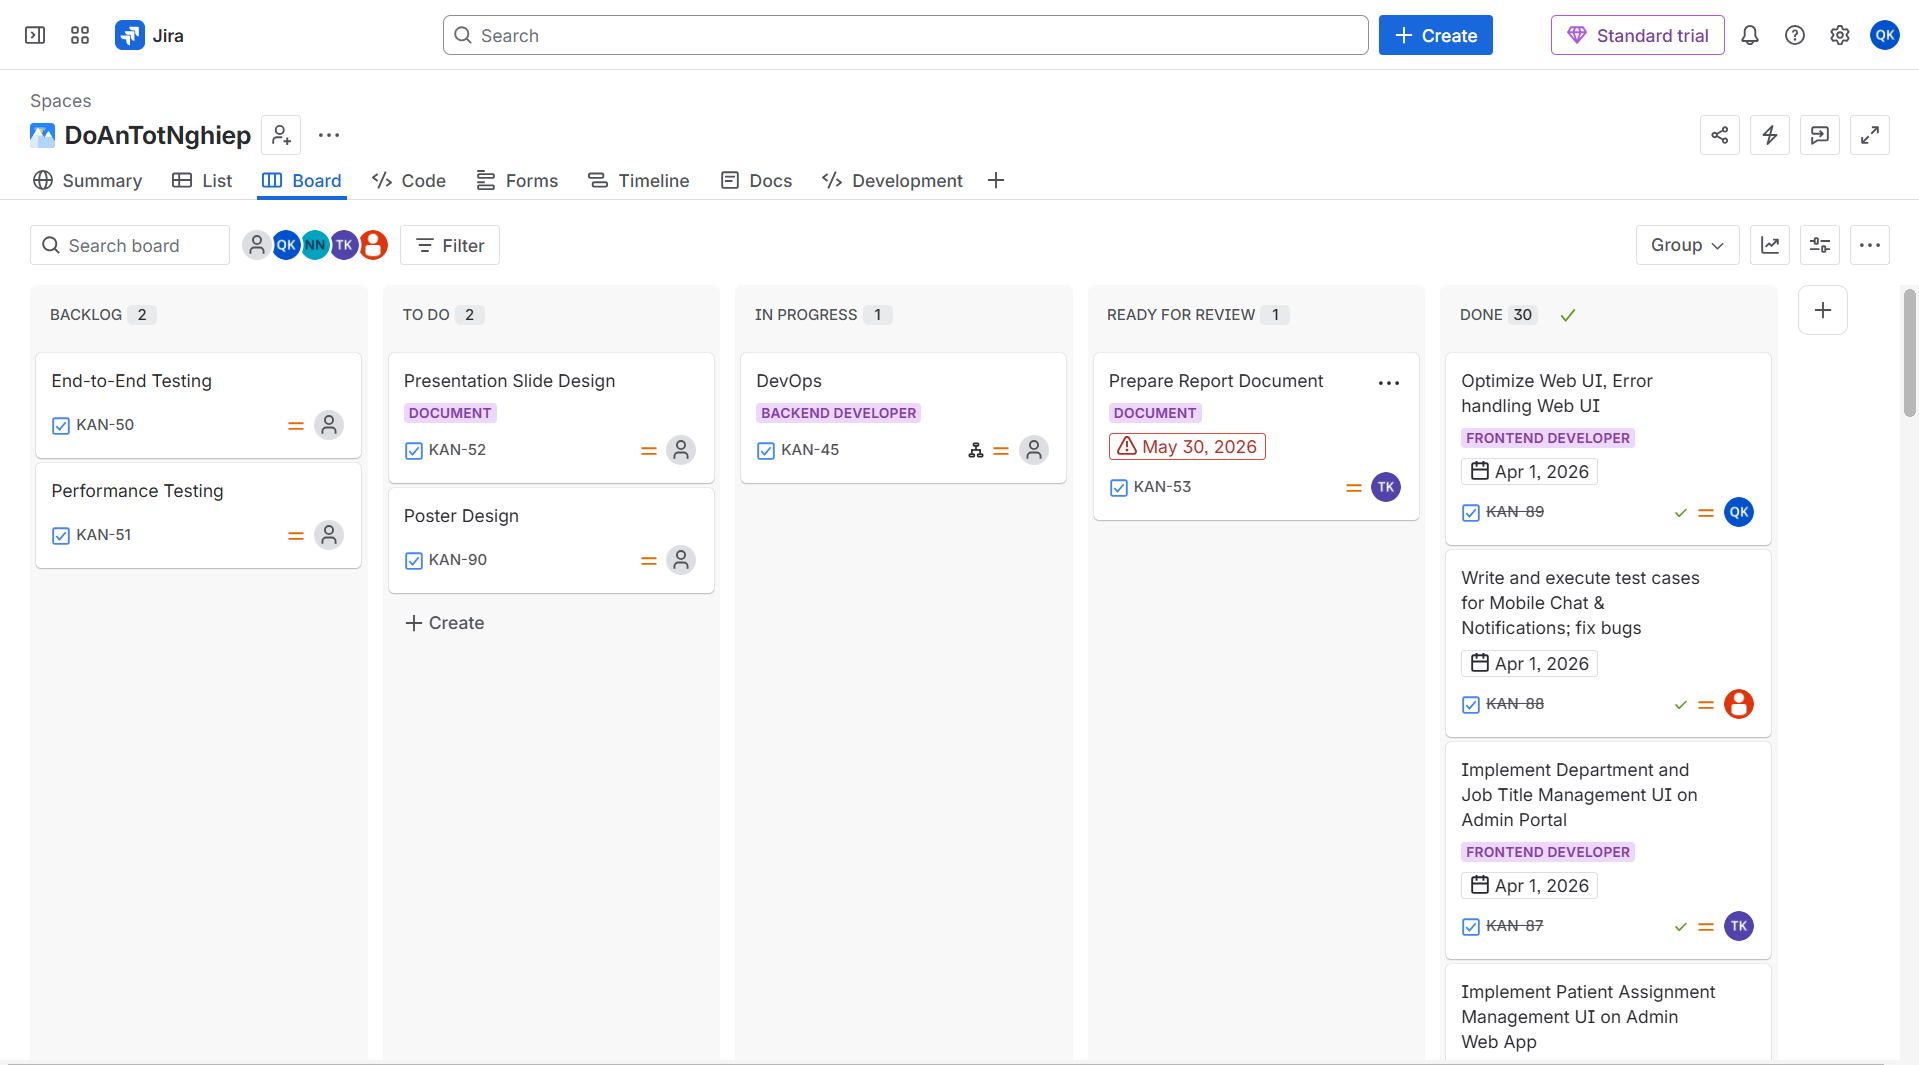
\includegraphics[width=\textwidth,keepaspectratio]{images/Chapter4/jira-sprint-board.png}
    \end{center}
    \caption{\textit{Danh sách công việc và phân chia nhiệm vụ của nhóm trên Jira}}
    \label{chapter4-image01}
    \end{figure}
\end{center}

\par Nhằm đảm bảo việc theo dõi tiến độ rõ ràng, nhóm thống nhất sử dụng các trạng thái chính sau trên Jira:
\begin{itemize}
    \item Backlog: Công việc đã được ghi nhận nhưng chưa được đưa vào sprint hiện tại. Các ticket ở trạng thái này có thể là ý tưởng chức năng mới, lỗi chưa cần xử lý ngay, yêu cầu cần làm rõ thêm hoặc các công việc thuộc giai đoạn sau của đồ án.
    \item To Do: Công việc đã đủ rõ để thực hiện và được đưa vào sprint hiện tại. Ticket ở trạng thái này cần có người phụ trách, mô tả yêu cầu và tiêu chí hoàn thành tương đối rõ ràng để thành viên có thể bắt đầu làm mà không phải hỏi lại quá nhiều thông tin cơ bản.
    \item In Progress: Công việc đang được thành viên phụ trách thực hiện. Trong trạng thái này, thành viên có thể cập nhật tiến độ, ghi chú khó khăn hoặc trao đổi thêm trong phần bình luận của ticket nếu phát hiện yêu cầu chưa rõ hoặc cần thay đổi so với kế hoạch ban đầu.
    \item Ready for Review: Công việc đã được cài đặt xong ở mức cơ bản và cần được các thành viên khác kiểm tra. Đối với backend, trạng thái này thường tương ứng với việc đã tạo pull request và cần review API. Đối với frontend hoặc mobile, trạng thái này có thể bao gồm việc kiểm tra giao diện, kiểm tra luồng thao tác và kiểm tra tích hợp với API.
    \item Done: Công việc đã hoàn thành, đã được kiểm tra và đạt yêu cầu đặt ra. Một ticket chỉ được chuyển sang Done khi chức năng hoạt động đúng trong luồng liên quan, mã nguồn đã được hợp nhất và không còn lỗi nghiêm trọng cần xử lý ngay.
\end{itemize}

\begin{center}
    \begin{figure}[H]
    \begin{center}
        % TODO: Bổ sung ảnh biểu đồ burndown/cumulative flow hoặc tiến độ sprint trên Jira
        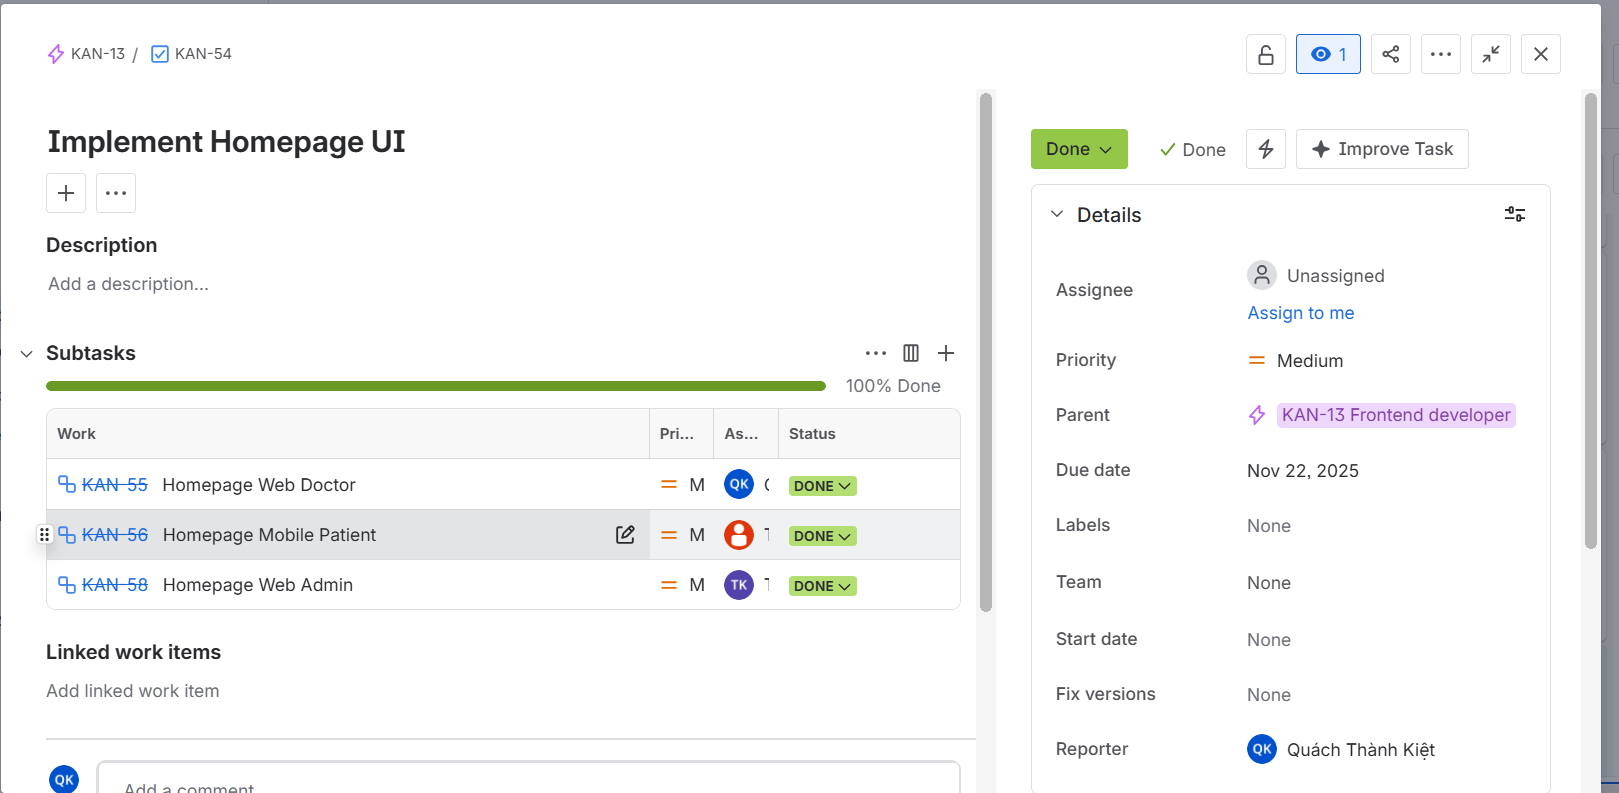
\includegraphics[width=\textwidth,keepaspectratio]{images/Chapter4/jira-sprint-progress.png}
    \end{center}
    \caption{\textit{Theo dõi tiến độ công việc dựa trên trạng thái ticket trong sprint}}
    \label{chapter4-image02}
    \end{figure}
\end{center}

\par Việc theo dõi tiến độ bằng Jira giúp nhóm phát hiện sớm các vấn đề trong sprint. Nếu một ticket ở trạng thái In Progress quá lâu, nhóm sẽ trao đổi trong buổi họp để xác định nguyên nhân, chẳng hạn như yêu cầu chưa rõ, API chưa hoàn thành, giao diện chưa có thiết kế, lỗi kỹ thuật khó xử lý hoặc thành viên phụ trách đang bị quá tải. Tùy tình huống, nhóm có thể chia nhỏ ticket, chuyển một phần công việc cho thành viên khác hoặc đưa ticket sang sprint sau nếu không còn phù hợp với mục tiêu hiện tại.

\section{Những khó khăn gặp phải}
\par Trong quá trình thực hiện đề tài, nhóm gặp nhiều khó khăn liên quan đến quy trình làm việc nhóm, thiết kế giao diện, xây dựng backend, phát triển ứng dụng di động, tích hợp frontend với API và triển khai hệ thống lên AWS. Do hệ thống có nhiều thành phần và nhiều vai trò người dùng, một thay đổi nhỏ ở backend có thể ảnh hưởng đến web bác sĩ, admin web và mobile app. Vì vậy, nhóm phải liên tục điều chỉnh cách làm việc, cải thiện giao tiếp và chuẩn hóa quy trình phát triển để hạn chế lỗi phát sinh trong quá trình tích hợp.

\subsection{Quá trình làm việc nhóm}

\subsubsection{Còn nhiều thiếu sót khi lên kế hoạch ở giai đoạn đầu}
\par Trong những tuần đầu, nhóm chưa ước lượng thật chính xác khối lượng công việc của từng chức năng. Một số chức năng ban đầu nhìn có vẻ đơn giản, chẳng hạn như nhập chỉ số sức khỏe hoặc hiển thị lịch sử đo, nhưng khi triển khai thực tế lại cần xử lý nhiều trường hợp hơn dự kiến như kiểm tra dữ liệu đầu vào, phân biệt loại chỉ số, tính MAP, xử lý thời điểm đo đường huyết, lưu dữ liệu, hiển thị biểu đồ và đồng bộ trạng thái giữa mobile với web bác sĩ. Điều này khiến một số ticket kéo dài hơn dự kiến và ảnh hưởng đến kế hoạch của sprint.

\par Ngoài ra, ở giai đoạn đầu, nhóm chưa mô tả đủ chi tiết một số yêu cầu trước khi giao việc. Ví dụ, một chức năng có thể chỉ được ghi là ``hiển thị cảnh báo'', nhưng chưa làm rõ cảnh báo hiển thị cho vai trò nào, lấy dữ liệu từ endpoint nào, có trạng thái đã xem hay chưa, có cần xác nhận hay không và khi nhấn vào cảnh báo thì điều hướng đến màn hình nào. Những thiếu sót này làm tăng thời gian trao đổi lại giữa các thành viên. Sau đó, nhóm đã cải thiện bằng cách yêu cầu mỗi ticket cần có mô tả rõ hơn, đặc biệt với các chức năng có sự liên kết giữa backend và frontend.

\subsubsection{Sự phụ thuộc giữa backend, frontend và mobile}
\par Một trong những khó khăn lớn của nhóm là sự phụ thuộc giữa các thành phần. Frontend và mobile cần API để hiển thị dữ liệu thật, trong khi backend cần biết giao diện cần những dữ liệu nào để thiết kế response phù hợp. Nếu backend thay đổi tên trường, thay đổi cấu trúc response hoặc thay đổi cách phân quyền mà không thông báo kịp thời, frontend và mobile có thể bị lỗi. Ngược lại, nếu frontend thay đổi cách hiển thị hoặc cần thêm dữ liệu mới, backend cũng phải điều chỉnh API.

\par Để giải quyết vấn đề này, nhóm dần hình thành thói quen thống nhất API contract trước khi bắt đầu cài đặt. Với các chức năng quan trọng, backend mô tả trước endpoint, method, request body, response mẫu và các mã lỗi có thể xảy ra. Frontend và mobile có thể dựa vào đó để cài đặt giao diện với dữ liệu giả trong thời gian chờ API hoàn thiện. Khi API đã hoàn thành, các thành viên chỉ cần thay dữ liệu giả bằng dữ liệu thật và kiểm thử tích hợp. Cách làm này giúp giảm thời gian chờ đợi giữa các mảng và tăng hiệu quả làm việc song song.

\subsubsection{Giao tiếp chưa thật sự hiệu quả trong một số thời điểm}
\par Do lịch học và lịch làm việc cá nhân của các thành viên không hoàn toàn giống nhau, nhóm đôi khi gặp khó khăn khi cần thảo luận gấp một vấn đề chung. Một số vấn đề kỹ thuật liên quan đến nhiều thành phần, ví dụ như lỗi xác thực, lỗi CORS, lỗi WebSocket hoặc lỗi thông báo, nếu chỉ trao đổi ngắn qua tin nhắn thì dễ hiểu sai nguyên nhân. Điều này khiến quá trình xử lý có lúc kéo dài hơn cần thiết.

\par Sau một thời gian, nhóm thống nhất rằng những vấn đề nhỏ có thể trao đổi trên Jira hoặc GitHub, nhưng những vấn đề liên quan đến nhiều thành phần sẽ được đưa vào buổi họp Google Meet để cùng xem trực tiếp. Việc chia sẻ màn hình, xem log, xem request/response và chạy thử luồng người dùng giúp nhóm xác định nguyên nhân nhanh hơn. Đồng thời, nhóm cũng cố gắng ghi lại các kết luận quan trọng sau mỗi buổi họp để tránh tình trạng đã thống nhất nhưng sau đó thành viên khác không nắm được.

\subsection{Thiết kế giao diện người dùng}

\subsubsection{Thiết kế giao diện trên ứng dụng di động}
\par Ứng dụng di động của hệ thống phục vụ chủ yếu cho bệnh nhân và y tá, trong đó bệnh nhân có thể là người lớn tuổi hoặc người không quen sử dụng các ứng dụng phức tạp. Vì vậy, giao diện mobile cần ưu tiên sự rõ ràng, thao tác đơn giản và hạn chế nhập sai dữ liệu. Trong giai đoạn đầu, một số màn hình nhập liệu còn có nhiều trường thông tin, nếu bố trí không hợp lý sẽ khiến người dùng khó phân biệt chỉ số nào là bắt buộc, chỉ số nào là tùy chọn và đơn vị đo của từng chỉ số là gì.

\par Bên cạnh đó, các chỉ số sức khỏe như huyết áp, đường huyết, nhịp tim, thân nhiệt, SpO2 đều có ý nghĩa khác nhau và cần được trình bày cẩn thận. Nếu giao diện chỉ hiển thị con số mà thiếu nhãn, thiếu đơn vị hoặc thiếu thông báo lỗi rõ ràng, người dùng có thể nhập nhầm hoặc hiểu nhầm dữ liệu. Để khắc phục, nhóm đã thiết kế lại các form nhập liệu theo hướng chia thành từng nhóm chỉ số, bổ sung nhãn, đơn vị, trạng thái lỗi và hướng dẫn ngắn gọn. Các màn hình lịch sử đo và cảnh báo cũng được cải thiện để người dùng dễ nhận biết chỉ số nào đang bất thường.

\subsubsection{Thiết kế giao diện trên nền tảng web}
\par Đối với ứng dụng web dành cho bác sĩ và trang quản trị, khó khăn lớn nhất là trình bày nhiều dữ liệu trên một màn hình mà vẫn đảm bảo dễ theo dõi. Bác sĩ cần xem danh sách bệnh nhân, thông tin chi tiết, lịch sử đo, biểu đồ xu hướng, cảnh báo, ngưỡng và nhắc nhở. Quản trị viên cần xem danh sách người dùng, khoa phòng, phân công và lịch sử hoạt động. Nếu bố cục không hợp lý, người dùng sẽ phải cuộn trang quá nhiều hoặc khó tìm thông tin quan trọng.

\par Nhóm đã sử dụng Figma để thử nhiều phương án bố cục trước khi cài đặt. Với các màn hình nhiều dữ liệu, nhóm ưu tiên sử dụng bảng, bộ lọc, ô tìm kiếm, thẻ thống kê và biểu đồ. Với các màn hình chi tiết bệnh nhân, nhóm cố gắng tách thông tin thành các khu vực như thông tin cá nhân, chỉ số gần nhất, biểu đồ xu hướng, cảnh báo và nhắc nhở. Việc thiết kế theo khu vực giúp bác sĩ dễ quan sát hơn và tránh cảm giác giao diện bị quá tải thông tin.

\subsection{Xây dựng backend và cơ sở dữ liệu}

\subsubsection{Thiết kế dữ liệu cho nhiều vai trò người dùng}
\par Backend của hệ thống cần hỗ trợ nhiều vai trò người dùng như bệnh nhân, bác sĩ, y tá và quản trị viên. Mỗi vai trò có các thông tin riêng và quyền truy cập khác nhau. Ví dụ, bệnh nhân có thông tin sức khỏe và dữ liệu đo, bác sĩ có chuyên khoa và danh sách bệnh nhân được phân công, y tá có thể hỗ trợ nhập liệu, còn quản trị viên có quyền quản lý hệ thống. Việc thiết kế model người dùng sao cho vừa dùng chung được các trường cơ bản, vừa mở rộng được theo vai trò là một trong những thách thức ở giai đoạn đầu.

\par Ngoài model người dùng, hệ thống còn cần nhiều collection khác như measurements, thresholds, alerts, reminders, assignments, departments, conversations, messages, notifications và activity logs. Các collection này có quan hệ nghiệp vụ với nhau, chẳng hạn một cảnh báo liên kết với bệnh nhân và lần đo, một nhắc nhở liên kết với bệnh nhân và bác sĩ tạo nhắc nhở, một hội thoại liên kết với bệnh nhân và bác sĩ, còn phân công quyết định bác sĩ hoặc y tá nào có quyền theo dõi bệnh nhân nào. Nhóm phải cân nhắc kỹ để tránh thiết kế dữ liệu quá rời rạc hoặc quá phụ thuộc lẫn nhau.

\subsubsection{Xử lý phân quyền và bảo mật dữ liệu sức khỏe}
\par Dữ liệu sức khỏe là dữ liệu nhạy cảm, do đó hệ thống cần kiểm soát quyền truy cập cẩn thận. Một bệnh nhân chỉ nên xem dữ liệu của chính mình, bác sĩ chỉ nên xem bệnh nhân được phân công, y tá chỉ nên thao tác trong phạm vi được giao, còn quản trị viên mới có quyền quản lý toàn bộ người dùng và phân công. Việc cài đặt phân quyền không chỉ dừng lại ở kiểm tra vai trò, mà còn cần kiểm tra quan hệ giữa người dùng hiện tại và tài nguyên đang truy cập.

\par Trong quá trình phát triển, nhóm nhận thấy một số API nếu chỉ kiểm tra JWT mà không kiểm tra quan hệ phân công có thể dẫn đến rủi ro truy cập dữ liệu ngoài phạm vi. Vì vậy, các API quan trọng cần được rà soát để đảm bảo kiểm tra đúng vai trò và đúng tài nguyên. Đây là một phần tương đối phức tạp vì mỗi nghiệp vụ có quy tắc khác nhau, ví dụ bác sĩ cấu hình ngưỡng cho bệnh nhân, y tá nhập chỉ số cho bệnh nhân, bệnh nhân xem cảnh báo của chính mình và quản trị viên phân công nhân viên y tế. Nhóm đã đưa các vấn đề phân quyền vào danh sách kiểm thử quan trọng trong giai đoạn hoàn thiện.

\subsubsection{Tích hợp Temporal, Redis, WebSocket và FCM}
\par Bên cạnh các API thông thường, backend còn tích hợp thêm nhiều thành phần hỗ trợ như Temporal để xử lý workflow, Redis để hỗ trợ Pub/Sub, WebSocket để cập nhật thời gian thực và Firebase Cloud Messaging để gửi push notification. Việc tích hợp các thành phần này giúp hệ thống có nhiều chức năng hơn, nhưng cũng làm tăng độ phức tạp khi debug. Một cảnh báo được tạo ra có thể đi qua nhiều bước: lưu measurement, chạy workflow, tạo alert, tạo notification, gửi FCM, publish sự kiện Redis và cập nhật WebSocket cho bác sĩ.

\par Khó khăn của nhóm là khi một bước trong chuỗi xử lý bị lỗi, cần xác định lỗi nằm ở đâu. Ví dụ, bệnh nhân không nhận được thông báo có thể do mobile chưa đăng ký token, backend lưu sai token, FCM trả lỗi, workflow chưa chạy hoặc notification đã được tạo nhưng chưa gửi. Để xử lý, nhóm phải kiểm tra log theo từng bước, bổ sung trạng thái gửi thông báo và kiểm thử từng thành phần riêng trước khi kiểm thử toàn bộ luồng. Qua quá trình này, nhóm học được cách thiết kế hệ thống theo hướng dễ quan sát hơn, hạn chế xử lý quá nhiều logic quan trọng trong một hàm duy nhất.

\subsection{Phát triển ứng dụng di động}

\subsubsection{Xử lý giao diện trên nhiều thiết bị}
\par Ứng dụng di động được phát triển bằng Expo và React Native, hướng đến khả năng chạy trên nhiều thiết bị khác nhau. Tuy nhiên, sự khác biệt về kích thước màn hình, tỷ lệ màn hình, hệ điều hành và cách hiển thị bàn phím khiến việc thiết kế giao diện gặp nhiều khó khăn. Một form nhập chỉ số có thể hiển thị tốt trên thiết bị màn hình lớn nhưng bị che nút lưu trên thiết bị màn hình nhỏ khi bàn phím xuất hiện. Các biểu đồ lịch sử đo cũng cần được điều chỉnh để không bị tràn hoặc quá nhỏ khi hiển thị trên các kích thước màn hình khác nhau.

\par Nhóm đã cố gắng thiết kế giao diện mobile theo hướng responsive, sử dụng scroll view khi cần, hạn chế chiều cao cố định quá cứng và kiểm tra các màn hình quan trọng trên nhiều thiết bị hoặc giả lập khác nhau. Đối với các màn hình nhập liệu, nhóm ưu tiên bố trí các trường theo chiều dọc, bổ sung khoảng cách hợp lý và đảm bảo nút thao tác chính luôn dễ nhìn. Đối với các màn hình biểu đồ hoặc lịch sử, nhóm cân nhắc cách hiển thị sao cho người dùng vẫn đọc được dữ liệu mà không cần thao tác phức tạp.

\subsubsection{Tích hợp thông báo đẩy trên mobile}
\par Thông báo đẩy là một chức năng quan trọng vì bệnh nhân cần được thông báo khi có cảnh báo hoặc nhắc nhở. Tuy nhiên, việc tích hợp thông báo đẩy không chỉ là hiển thị một notification trên thiết bị, mà còn cần xử lý quyền nhận thông báo, lấy token thiết bị, gửi token về backend, lưu token theo người dùng và thiết bị, xử lý khi token thay đổi, xử lý khi người dùng đăng xuất và xử lý điều hướng khi người dùng nhấn vào thông báo.

\par Trong quá trình phát triển, nhóm gặp khó khăn khi kiểm thử thông báo trên các môi trường khác nhau. Thông báo có thể hoạt động khác nhau giữa simulator, emulator và thiết bị thật, đồng thời cũng phụ thuộc vào cấu hình Firebase, quyền của ứng dụng và nền tảng hệ điều hành. Nhóm đã tách riêng chức năng đăng ký token, lưu token và gửi thông báo để dễ kiểm tra từng phần. Đối với phạm vi đồ án, nhóm ưu tiên đảm bảo thông báo hoạt động tốt trong kịch bản demo chính, đồng thời ghi nhận các hạn chế để cải thiện ở giai đoạn sau.

\subsection{Phát triển frontend web}

\subsubsection{Tích hợp API và xử lý trạng thái giao diện}
\par Ứng dụng web dành cho bác sĩ và trang quản trị có nhiều màn hình cần gọi API, hiển thị dữ liệu bảng, biểu đồ và form nhập liệu. Khó khăn của frontend không chỉ nằm ở việc dựng giao diện đúng theo Figma, mà còn nằm ở việc xử lý đầy đủ các trạng thái khi gọi API. Mỗi màn hình cần xử lý trạng thái đang tải, lỗi kết nối, dữ liệu rỗng, dữ liệu hợp lệ, lỗi xác thực, lỗi phân quyền và trường hợp token hết hạn. Nếu không xử lý đầy đủ, giao diện có thể bị trắng, hiển thị dữ liệu cũ hoặc khiến người dùng không biết thao tác tiếp theo là gì.

\par Nhóm đã sử dụng các service API riêng cho từng nghiệp vụ và cấu hình interceptor để hỗ trợ xử lý phiên đăng nhập. Khi backend trả về lỗi, frontend cần hiển thị thông báo phù hợp thay vì chỉ ghi log ở console. Đối với các bảng dữ liệu, nhóm bổ sung tìm kiếm, phân trang hoặc bộ lọc ở những màn hình cần thiết. Đối với biểu đồ, nhóm cần chuyển đổi dữ liệu đo từ backend sang dạng phù hợp với thư viện biểu đồ, đồng thời xử lý trường hợp bệnh nhân chưa có dữ liệu hoặc dữ liệu không đủ để vẽ xu hướng.

\subsubsection{Đảm bảo tính nhất quán giữa web bác sĩ và admin web}
\par Web bác sĩ và admin web phục vụ hai nhóm người dùng khác nhau nhưng vẫn cần có sự nhất quán về phong cách giao diện, cách dùng màu sắc, kích thước chữ, button, bảng dữ liệu và form nhập liệu. Trong giai đoạn đầu, khi Khoa và Kiệt phát triển song song nhiều màn hình, một số component có thể bị viết lặp lại hoặc có cách hiển thị chưa thống nhất. Điều này làm cho giao diện thiếu đồng bộ và khó bảo trì khi cần thay đổi style chung.

\par Để cải thiện, nhóm dần tách các thành phần giao diện dùng chung như button, input, modal, table, card, layout và sidebar. Việc tái sử dụng component giúp giảm số lượng mã nguồn lặp, đồng thời đảm bảo khi cần chỉnh sửa giao diện, nhóm chỉ cần cập nhật ở một nơi. Ngoài ra, các thành viên frontend cũng thường xuyên kiểm tra chéo giao diện của nhau trong buổi họp để phát hiện sớm các điểm chưa thống nhất.

\subsection{Triển khai hệ thống trên AWS}

\subsubsection{Cấu hình backend trên AWS EC2}
\par Nhóm triển khai backend trên AWS EC2 bằng Docker Compose. Cách triển khai này giúp nhóm chủ động quản lý các service như API server, worker, Redis, Temporal và Nginx trên cùng một máy chủ. Tuy nhiên, việc triển khai thực tế phức tạp hơn so với chạy local vì cần cấu hình security group, domain hoặc địa chỉ public, biến môi trường production, network giữa các container, volume lưu dữ liệu, log container và cơ chế khởi động lại khi server gặp sự cố.

\par Một số lỗi chỉ xuất hiện khi deploy lên EC2, chẳng hạn như API không truy cập được do chưa mở cổng, WebSocket không hoạt động do thiếu cấu hình reverse proxy, frontend gọi API bị chặn bởi CORS hoặc backend không kết nối được đến dịch vụ bên ngoài do thiếu biến môi trường. Để xử lý, nhóm phải kiểm tra lần lượt từ tầng mạng, Nginx, container, log ứng dụng đến cấu hình API. Quá trình này tốn thời gian nhưng giúp nhóm hiểu rõ hơn về hạ tầng triển khai và các vấn đề thường gặp khi đưa ứng dụng lên môi trường internet.

\subsubsection{Triển khai web bác sĩ và admin web trên Amazon S3}
\par Ứng dụng web bác sĩ và trang quản trị được build thành static files và triển khai lên Amazon S3. So với việc chạy web trực tiếp trên EC2, cách triển khai này giúp tách biệt frontend và backend rõ ràng hơn. Frontend chỉ cần lưu trữ và phục vụ các file tĩnh, trong khi backend tập trung xử lý API. Tuy nhiên, khi triển khai Single Page Application trên S3, nhóm cần chú ý cấu hình đường dẫn, file index, biến môi trường \texttt{VITE\_API\_URL} và cách ứng dụng xử lý route khi người dùng refresh trang.

\par Ngoài ra, quá trình deploy frontend cũng cần đồng bộ với backend. Nếu frontend đã được build với URL API cũ hoặc backend chưa deploy endpoint mới, ứng dụng có thể bị lỗi sau khi đưa lên S3. Vì vậy, nhóm sử dụng GitHub Actions để giảm thao tác thủ công và đảm bảo quá trình build sử dụng đúng biến môi trường production. Khi có thay đổi lớn ở API, nhóm cần kiểm tra lại cả web bác sĩ và admin web sau khi deploy để đảm bảo không có lỗi tích hợp.

\subsubsection{Quản lý cấu hình và thông tin nhạy cảm}
\par Khi triển khai hệ thống, nhóm nhận thấy việc quản lý biến môi trường và thông tin nhạy cảm là vấn đề rất quan trọng. Backend cần nhiều thông tin cấu hình như chuỗi kết nối MongoDB, JWT secret, cấu hình Redis, Temporal, Cloudinary, Firebase, OAuth và các biến môi trường liên quan đến domain. Nếu các thông tin này bị đưa trực tiếp vào mã nguồn hoặc commit lên repository, hệ thống có thể gặp rủi ro bảo mật nghiêm trọng.

\par Để hạn chế rủi ro, nhóm cần tách cấu hình production ra khỏi mã nguồn và sử dụng GitHub Secrets hoặc file môi trường trên server khi triển khai. Các file chứa token, cookie, mật khẩu hoặc thông tin đăng nhập demo không nên được đưa vào repository chính thức. Đây là một bài học quan trọng trong quá trình triển khai, đặc biệt với hệ thống xử lý thông tin cá nhân và dữ liệu sức khỏe của người dùng.

\subsection{Kiểm thử và hoàn thiện sản phẩm}

\subsubsection{Kiểm thử theo vai trò người dùng}
\par Vì hệ thống có nhiều vai trò khác nhau, nhóm không thể chỉ kiểm thử từng chức năng riêng lẻ mà cần kiểm thử theo luồng sử dụng của từng vai trò. Với bệnh nhân, các luồng chính gồm đăng nhập, nhập chỉ số, xem lịch sử, nhận cảnh báo, nhận nhắc nhở, xem thông báo và chat với bác sĩ. Với bác sĩ, các luồng chính gồm xem danh sách bệnh nhân, xem chi tiết bệnh nhân, cấu hình ngưỡng, xem cảnh báo, xác nhận cảnh báo, tạo nhắc nhở và chat với bệnh nhân. Với y tá, nhóm kiểm thử luồng xem bệnh nhân được phân công và nhập chỉ số hỗ trợ. Với quản trị viên, nhóm kiểm thử quản lý người dùng, khoa phòng, phân công và xem lịch sử hoạt động.

\par Kiểm thử theo vai trò giúp nhóm phát hiện các lỗi phân quyền và lỗi luồng nghiệp vụ dễ hơn. Ví dụ, một API có thể hoạt động đúng khi gọi bằng tài khoản admin nhưng không hoạt động với tài khoản bác sĩ, hoặc một dữ liệu hiển thị đúng trên web nhưng bệnh nhân không nhận được thông báo trên mobile. Nhóm ghi nhận các lỗi phát hiện được vào Jira, phân loại mức độ ưu tiên và xử lý theo sprint. Những lỗi ảnh hưởng đến demo hoặc luồng chính được ưu tiên sửa trước.

\subsubsection{Kiểm thử tích hợp giữa các thành phần}
\par Ngoài kiểm thử theo vai trò, nhóm cũng thực hiện kiểm thử tích hợp giữa các thành phần của hệ thống. Một số chức năng như cảnh báo, nhắc nhở và chat có sự tham gia của nhiều thành phần cùng lúc, nên không thể kiểm thử riêng lẻ từng phần. Ví dụ, chức năng cảnh báo cần kiểm tra mobile gửi measurement, backend lưu dữ liệu, workflow tạo alert, notification được lưu, FCM gửi thông báo và web bác sĩ cập nhật cảnh báo. Nếu chỉ kiểm thử API tạo measurement mà không kiểm tra phần còn lại, nhóm có thể bỏ sót lỗi trong workflow hoặc notification.

\par Quá trình kiểm thử tích hợp giúp nhóm phát hiện các lỗi liên quan đến thời gian thực, đồng bộ trạng thái và cấu hình môi trường. Một số lỗi chỉ xảy ra khi chạy trên môi trường deploy thật, chẳng hạn WebSocket bị proxy sai header, push notification không gửi do token không hợp lệ hoặc frontend gọi nhầm URL API. Nhóm đã sử dụng log server, log trình duyệt, log mobile và dữ liệu trong MongoDB để đối chiếu kết quả, từ đó xác định lỗi nằm ở thành phần nào.

\subsection{Bài học kinh nghiệm}
\par Qua quá trình thực hiện đề tài, nhóm rút ra rằng đối với một hệ thống có nhiều thành phần, việc lập kế hoạch và mô tả yêu cầu rõ ràng quan trọng không kém việc viết mã nguồn. Nếu yêu cầu không rõ, backend, frontend và mobile rất dễ phát triển lệch nhau, dẫn đến mất nhiều thời gian chỉnh sửa khi tích hợp. Vì vậy, nhóm cần có thói quen viết ticket chi tiết, thống nhất API contract, cập nhật tài liệu và demo thường xuyên để phát hiện vấn đề sớm.

\par Nhóm cũng nhận thấy việc quản lý mã nguồn bằng pull request và code review giúp cải thiện chất lượng sản phẩm rõ rệt. Khi có thành viên khác đọc lại mã nguồn, nhiều lỗi tiềm ẩn có thể được phát hiện trước khi merge vào nhánh chính. Ngoài ra, việc chia nhỏ chức năng, tách module và giữ cấu trúc mã nguồn rõ ràng giúp nhóm dễ sửa lỗi hơn khi hệ thống ngày càng lớn. Đây là kinh nghiệm quan trọng cho các dự án phần mềm thực tế, nơi sản phẩm cần được bảo trì và mở rộng trong thời gian dài.

\par Cuối cùng, quá trình triển khai lên AWS giúp nhóm hiểu rằng một ứng dụng chạy được ở local chưa chắc đã vận hành tốt ở môi trường production. Các vấn đề về biến môi trường, HTTPS, CORS, reverse proxy, WebSocket, Docker, security group và secret management đều cần được chuẩn bị cẩn thận. Những kinh nghiệm này giúp nhóm không chỉ hoàn thành đồ án mà còn có thêm hiểu biết thực tế về quy trình phát triển, triển khai và vận hành một hệ thống phần mềm hoàn chỉnh.